% ============================================================
%  3D_PROJECT_REPORT.tex — Quadruped Robot Development Report
%  Engine  : XeLaTeX (compile TWICE for TOC)
%  Group   : Group-E, CGEC ECE 2027
% ============================================================

\documentclass[12pt, a4paper]{article}

% ── Geometry ──────────────────────────────────────────────
\usepackage[a4paper, margin=0.8in]{geometry}

% ── Fonts (XeLaTeX only) ─────────────────────────────────
\usepackage{fontspec}
\usepackage{unicode-math}
\setmainfont{TeX Gyre Pagella}
\setmonofont[Scale=0.88]{TeX Gyre Cursor}
\setmathfont{Latin Modern Math}
% Devanagari font for college motto (Nirmala UI ships with Windows)
\newfontfamily\devanagarifont{Nirmala UI}[Scale=0.95]

% ── Spacing ───────────────────────────────────────────────
\usepackage{setspace}
\usepackage{parskip}
\setlength{\parindent}{0pt}
\setlength{\parskip}{8pt}
\onehalfspacing

% ── No hyphenation ────────────────────────────────────────
\usepackage[none]{hyphenat}
\sloppy

% ── Colours ───────────────────────────────────────────────
\usepackage{xcolor}
\definecolor{myred}{RGB}{200,0,0}
\definecolor{myblue}{RGB}{0,50,160}
\definecolor{mygreen}{RGB}{0,140,70}
\definecolor{myteal}{RGB}{0,130,130}
\definecolor{myamber}{RGB}{180,100,0}
\definecolor{mypurple}{RGB}{110,0,160}
\definecolor{codebg}{RGB}{246,248,250}
\definecolor{codecomment}{RGB}{106,153,85}
\definecolor{codeborder}{RGB}{208,215,222}
\definecolor{footergray}{RGB}{150,150,150}

% ── Section Title Styling ─────────────────────────────────
\usepackage{titlesec}
\titleformat{\section}
  {\Large\bfseries\color{myred}}{\thesection.}{0.5em}{}[\titlerule]
\titleformat{\subsection}
  {\normalsize\bfseries\color{myblue}}{\thesubsection.}{0.5em}{}
\titleformat{\subsubsection}
  {\normalsize\bfseries\color{mygreen}}{\thesubsubsection.}{0.5em}{}

% ── Header / Footer ───────────────────────────────────────
\usepackage{fancyhdr}
\pagestyle{fancy}
\fancyhf{}
\fancyfoot[C]{\small\thepage}
\renewcommand{\headrulewidth}{0pt}
\renewcommand{\footrulewidth}{0.4pt}
\fancypagestyle{plain}{%
  \fancyhf{}%
  \fancyfoot[C]{\small\thepage}%
  \renewcommand{\headrulewidth}{0pt}%
  \renewcommand{\footrulewidth}{0.4pt}%
}

% ── Graphics ──────────────────────────────────────────────
\usepackage{graphicx}
\usepackage{caption}
\usepackage{float}

% ── Tables ────────────────────────────────────────────────
\usepackage{booktabs}
\usepackage{tabularx}
\usepackage{array}
\usepackage{colortbl}
\renewcommand{\arraystretch}{1.3}

% ── Lists ─────────────────────────────────────────────────
\usepackage{enumitem}

% ── Code Listings ─────────────────────────────────────────
\usepackage{listings}
\lstset{
  backgroundcolor=\color{codebg},
  basicstyle=\ttfamily\small,
  commentstyle=\color{codecomment}\itshape,
  keywordstyle=\color{myblue}\bfseries,
  stringstyle=\color{myred},
  frame=single,
  rulecolor=\color{codeborder},
  breaklines=true,
  numbers=left,
  numberstyle=\tiny\color{footergray},
  tabsize=2,
  captionpos=b,
  xleftmargin=1.5em,
  framexleftmargin=1.5em
}

% ── TikZ ──────────────────────────────────────────────────
\usepackage{tikz}
\usepackage{pgfplots}
\usetikzlibrary{shapes.geometric,arrows.meta,positioning,calc,fit,backgrounds}
\pgfplotsset{compat=1.18}

% ── tcolorbox ─────────────────────────────────────────────
\usepackage{tcolorbox}
\tcbuselibrary{skins,breakable}

% ── Hyperref + bookmark (bookmark replaces .out, stops loop)
\usepackage[colorlinks=true,
            linkcolor=myblue,
            urlcolor=myteal,
            citecolor=mygreen,
            pdftitle={Report of Quadruped Robot Development},
            pdfauthor={Group-E CGEC ECE 2027},
            pdfsubject={WTL MeitY Industrial Training Report}]{hyperref}
\usepackage{bookmark}

% ─────────────────────────────────────────────────────────
%  DOCUMENT
% ─────────────────────────────────────────────────────────
\begin{document}

% Front matter: Roman page numbers
\pagenumbering{roman}

% ============================================================
%  1. COVER PAGE
% ============================================================
\begin{titlepage}
\thispagestyle{empty}
\centering
\vspace*{2cm}
{\Huge\bfseries\color{myred} 3D PRINTING \&\par}
\vspace{0.3cm}
{\Huge\bfseries\color{myred} ADDITIVE MANUFACTURING TECHNOLOGY\par}
\vspace{0.8cm}
{\Large\bfseries\color{myblue} Quadruped Robot Development Report\par}
\vspace{0.5cm}
{\large\color{myamber}\textit{Report of Quadruped Robot Development}\par}
\vspace{1cm}
\vspace{10cm}   % reserved for cover photo
\vfill
{\large Department of Electronics and Communication Engineering\par}
{\large Cooch Behar Government Engineering College\par}
\vspace{0.3cm}
{\large\bfseries 2026\par}
\end{titlepage}

% ============================================================
%  2. CERTIFICATE OF APPROVAL
% ============================================================
\newpage
\thispagestyle{plain}

\begin{center}
  {\Large\bfseries\color{myred} Certificate of Approval\par}
\end{center}
\addcontentsline{toc}{section}{Certificate of Approval}

\vspace{0.8cm}

It is hereby approved that the project report entitled
\textbf{Report of Quadruped Robot Development} submitted by:

\vspace{0.3cm}
\begin{enumerate}[label=\arabic*., leftmargin=2.5em, itemsep=6pt]
  \item SARUPYA GUHA \hfill (Roll No.: 34900323046 / Reg. ID: FS08A0198)
  \item SOHAN GHOSH \hfill (Roll No.: 34900323050 / Reg. ID: FS08A0202)
  \item SAYAN SARKAR \hfill (Roll No.: 34900323048 / Reg. ID: FS08A0157)
  \item DEBANJAN CHAKRABORTY \hfill (Roll No.: 34900323015 / Reg. ID: FS08A0154)
  \item JOYDIP DAS \hfill (Roll No.: 34900323020 / Reg. ID: FS08A0220)
  \item AUSHI SARKAR \hfill (Roll No.: 34900323011 / Reg. ID: FS08A0288)
  \item ANUPAM DUTTA \hfill (Roll No.: 34900323003 / Reg. ID: FS08A0206)
  \item BIKKRAM DAS \hfill (Roll No.: 34900323012 / Reg. ID: FS08A0528)
  \item BIRAJ SARKAR \hfill (Roll No.: 34900323013 / Reg. ID: FS08A0239)
  \item SOUMYAJIT PANDIT \hfill (Roll No.: 34900323052 / Reg. ID: FS08A0189)
\end{enumerate}

\vspace{0.5cm}

As part of their certification-based industrial training in
\textbf{Robotics \& Embedded Systems}, conducted under the supervision of
\textbf{WTL \& MeitY, Cooch Behar Government Engineering College},
Cooch Behar, West Bengal.

\vspace{3.5cm}

\noindent
\begin{tabular}{p{8cm} p{7cm}}
  \rule{7cm}{0.4pt} & \rule{7cm}{0.4pt} \\[5pt]
  Dr.\ Palash Das                  & Mrs.\ Susmita Banik Barik \\
  (HOD, Dept.\ of ECE, CGEC)       & (Project Engineer, WTL, MeitY)
\end{tabular}

\vfill

% ============================================================
%  3. TITLE PAGE  — single page, all content fits
% ============================================================
\newpage
\thispagestyle{plain}

\begin{center}

{\LARGE\bfseries\color{myred} REPORT FOR QUADRUPED ROBOT DEVELOPMENT\par}
\vspace{0.3cm}
{\small\color{myblue} Certification-Based Industrial Training\par}
{\small\color{myblue} WTL \& MeitY Project, CGEC\par}

\vspace{0.5cm}
{\normalsize\bfseries Submitted by:\par}
\vspace{0.3cm}

{\small\bfseries SARUPYA GUHA} {\small (Roll No.: 34900323046 / Reg. ID: FS08A0198)}\\[3pt]
{\small\bfseries SOHAN GHOSH} {\small (Roll No.: 34900323050 / Reg. ID: FS08A0202)}\\[3pt]
{\small\bfseries SAYAN SARKAR} {\small (Roll No.: 34900323048 / Reg. ID: FS08A0157)}\\[3pt]
{\small\bfseries DEBANJAN CHAKRABORTY} {\small (Roll No.: 34900323015 / Reg. ID: FS08A0154)}\\[3pt]
{\small\bfseries JOYDIP DAS} {\small (Roll No.: 34900323020 / Reg. ID: FS08A0220)}\\[3pt]
{\small\bfseries AUSHI SARKAR} {\small (Roll No.: 34900323011 / Reg. ID: FS08A0288)}\\[3pt]
{\small\bfseries ANUPAM DUTTA} {\small (Roll No.: 34900323003 / Reg. ID: FS08A0206)}\\[3pt]
{\small\bfseries BIKKRAM DAS} {\small (Roll No.: 34900323012 / Reg. ID: FS08A0528)}\\[3pt]
{\small\bfseries BIRAJ SARKAR} {\small (Roll No.: 34900323013 / Reg. ID: FS08A0239)}\\[3pt]
{\small\bfseries SOUMYAJIT PANDIT} {\small (Roll No.: 34900323052 / Reg. ID: FS08A0189)}\\[3pt]

\vspace{0.3cm}
{\normalsize\bfseries\color{myblue} Group-E\par}

\vspace{0.4cm}
{\normalsize\bfseries Under the guidance of:\par}
\vspace{0.2cm}

{\small\bfseries Dr.\ PALASH DAS}\\[-1pt]
{\small (HOD of ECE Dept., CGEC)}\\[3pt]
{\small\bfseries Mrs.\ SUSMITA BANIK BARIK}\\[-1pt]
{\small (Project Eng., WTL \& MeitY Project)}\\[3pt]
{\small\bfseries Mr.\ ARIJIT BHUNIA}\\[-1pt]
{\small (Project Co-ordinator, WTL \& MeitY Project)}\\[3pt]
{\small\bfseries Mr.\ BHASKAR MONDAL}\\[-1pt]
{\small (Faculty, WTL \& MeitY Project)}\\[5pt]

\vspace{0.3cm}
{\small Cooch Behar Government Engineering College}\\[2pt]
{\small Department of Electronics and Communication Engineering}\\[4pt]
{\normalsize\bfseries 2026}

\end{center}
%  4. ACKNOWLEDGEMENT
% ============================================================
\newpage
\thispagestyle{fancy}

\section*{\color{myred}Acknowledgement}
\addcontentsline{toc}{section}{Acknowledgement}

We, the students of Group-E, Department of Electronics and Communication
Engineering, Cooch Behar Government Engineering College, would like to express
our heartfelt gratitude to everyone who supported us throughout the development
of this Quadruped Robot project.

First and foremost, we extend our sincere thanks to \textbf{Dr.\ Palash Das},
Head of the Department of ECE, CGEC, for his invaluable guidance in
\textbf{embedded systems and robotics}, constant encouragement, and providing
us with the resources required to carry out this project. His expert knowledge
in electronics and microcontroller-based systems helped us at every phase of
the robot development, and his vision for integrating cutting-edge technology
into the curriculum has been a constant source of inspiration.

We are deeply grateful to \textbf{Mrs.\ Susmita Banik Barik}, Project Engineer,
WTL \& MeitY Project, for her expert mentorship in \textbf{3D printing and
additive manufacturing}. Her hands-on guidance in FDM printing, material
selection, and slicer settings enabled us to successfully fabricate all
chassis components of the robot. We also sincerely thank
\textbf{Mr.\ Arijit Bhunia}, Project Co-ordinator, and \textbf{Mr.\ Bhaskar
Mondal}, Faculty, WTL \& MeitY Project, for their regular feedback and patient
guidance during every phase of development.

We are thankful to the \textbf{Government of India, Ministry of Electronics and
Information Technology (MeitY)}, and the \textbf{World Trade Learning (WTL)}
initiative for sponsoring this industrial training programme. We acknowledge the
excellent facilities at the \textbf{CGEC 3D Printing Lab} --- the air-conditioned
workspace, smart board, modern computers, FDM 3D printers, and the fully equipped
electronics lab --- which made hands-on learning truly possible. Finally, we thank
every member of Group-E for their collaborative spirit, patience, and dedication
throughout this project.

% ============================================================
%  5. TABLE OF CONTENTS
% ============================================================
\newpage
\tableofcontents
\newpage

% Switch to Arabic numbering from here
\pagenumbering{arabic}
\setcounter{page}{1}

% ============================================================
%  1. 3D PRINTING --- THEORY & PROCESS
% ============================================================
\section{3D Printing Process}

\subsection{What is Additive Manufacturing?}

Additive Manufacturing (AM) is a process of building a three-dimensional object
by depositing material layer-by-layer directly from a digital model, as opposed
to subtractive manufacturing which removes material from a solid block. AM
enables fabrication of complex geometries that are difficult or impossible to
produce by conventional methods, with minimal material waste.

\subsubsection{Types of Additive Manufacturing}

\begin{itemize}[itemsep=4pt]

  \item \textbf{Vat Photopolymerization (SLA / DLP)} --- A liquid photopolymer
  resin is selectively cured by a UV light source (laser or digital projector)
  layer by layer. The build platform moves upward (or downward in bottom-up
  systems) after each layer. Produces very high resolution parts but resins are
  brittle and sensitive to UV degradation. Used in jewellery, dental, and
  prototyping.

  \item \textbf{Powder Bed Fusion (SLS / SLM / DMLS)} --- A thin layer of
  powder (polymer, metal, or ceramic) is spread across a build platform and a
  laser or electron beam fuses the powder at selected points. Unfused powder
  acts as support. SLS uses nylon/PA12; SLM/DMLS use metal alloys such as
  titanium and stainless steel. Used extensively in aerospace, medical implants,
  and high-performance engineering parts.

  \item \textbf{Fused Deposition Modelling (FDM / FFF)} --- A thermoplastic
  filament is fed through a heated nozzle and deposited in a predetermined path
  on the build platform, bonding to the previous layer as it cools. This is the
  most widely used AM process for education and prototyping due to its low cost,
  ease of use, and wide range of compatible materials. \textbf{All parts in this
  project were printed using FDM.}

  \item \textbf{Material Jetting} --- Droplets of photopolymer are jetted onto
  the build surface and cured immediately by UV. Allows multi-material and
  full-colour prints. High accuracy but expensive.

  \item \textbf{Binder Jetting} --- A liquid binder is selectively deposited
  onto a powder bed to join particles. No heat is applied during printing;
  a post-process sintering step densifies the part. Used for sand casting moulds
  and metal parts.

  \item \textbf{Directed Energy Deposition (DED)} --- A focused energy source
  (laser or electron beam) melts material (wire or powder) as it is deposited.
  Mainly used for repairing or adding features to existing metal components.

\end{itemize}

\subsection{Subtractive Manufacturing --- A Brief Overview}

Unlike additive manufacturing, subtractive manufacturing starts with a solid
block (workpiece) and removes material using cutting tools to achieve the
desired shape. Key processes include:

\begin{itemize}[itemsep=3pt]
  \item \textbf{CNC Milling} --- A rotating multi-point cutter removes material
  along multiple axes. Produces flat surfaces, slots, and complex 3D contours
  in metal, wood, and plastic.
  \item \textbf{CNC Turning (Lathe)} --- The workpiece rotates against a fixed
  cutting tool. Used for cylindrical parts such as shafts, bushings, and
  threaded components.
  \item \textbf{Drilling} --- A rotating drill bit creates holes of defined
  diameter and depth.
  \item \textbf{Grinding} --- An abrasive wheel removes small amounts of
  material for high surface finish and tight tolerances.
  \item \textbf{EDM (Electrical Discharge Machining)} --- Material is removed
  by controlled electrical sparks between electrode and workpiece. Used for
  hardened metals and complex cavities.
\end{itemize}

Compared to subtractive methods, FDM 3D printing requires no fixturing, produces
no chips, and can create internal cavities freely --- making it ideal for rapid
prototyping of robot chassis components.

\subsection{3D File Formats}

A 3D model must be saved in a compatible file format before it can be sliced and
printed. Common formats include:

\begin{itemize}[itemsep=4pt]
  \item \textbf{STL (Standard Triangle Language / Standard Tessellation
  Language)} --- Represents the surface geometry of a 3D object as a collection
  of linked triangles (tessellation). Each triangle is defined by three vertices
  and a normal vector. STL files are simple, widely supported, and easily
  understood by 3D printers. They do not store colour, texture, or material
  information. \textbf{In our training, we exclusively use \texttt{.stl} files}
  exported from FreeCAD for all printed parts.

  \item \textbf{OBJ (Wavefront OBJ)} --- A text-based format storing vertices,
  normals, texture coordinates, and polygon faces. Supports colour and texture
  via an associated \texttt{.mtl} material file. More complex than STL but
  better suited for visual rendering and multi-colour models.

  \item \textbf{VRML / X3D (.wrl / .x3d)} --- Virtual Reality Modelling
  Language. Stores 3D geometry along with colour, texture, and scene
  information. Used for interactive 3D web content and full-colour printing on
  specialised printers.

  \item \textbf{3MF (3D Manufacturing Format)} --- A modern XML-based format
  developed by Microsoft and industry partners. Stores geometry, colour,
  material, and print settings in a single file. Increasingly adopted as a
  replacement for STL in professional workflows.

  \item \textbf{STEP / IGES} --- CAD exchange formats that store precise
  parametric geometry (B-rep). Used for engineering data exchange between CAD
  packages, not directly by slicers.
\end{itemize}

\subsection{3D Printing Workflow}

The complete workflow from design to physical part involves the following stages:

\vspace{0.3cm}
\begin{tcolorbox}[
  colback=gray!15, colframe=gray!40, arc=4pt, boxrule=0.5pt,
  title={\bfseries\color{myblue} 3D Printing Workflow}
]
\centering
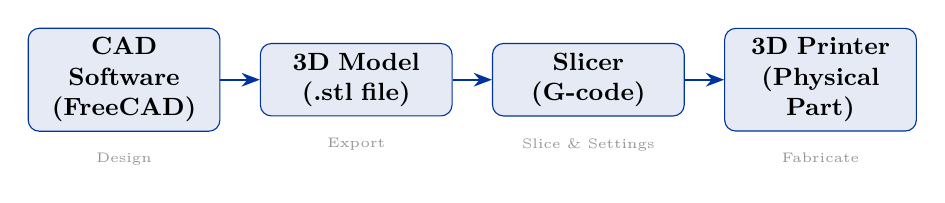
\begin{tikzpicture}[
  node distance=0.4cm and 0.5cm,
  box/.style={rectangle, draw=myblue, fill=myblue!10, rounded corners=4pt,
              text width=2.2cm, text centered, minimum height=0.8cm,
              font=\small\bfseries},
  arr/.style={thick, ->, >=Stealth, color=myblue}
]
  \node[box] (a) {CAD Software\\(FreeCAD)};
  \node[box, right=of a] (b) {3D Model\\(.stl file)};
  \node[box, right=of b] (c) {Slicer\\(G-code)};
  \node[box, right=of c] (d) {3D Printer\\(Physical Part)};
  \draw[arr] (a)--(b); \draw[arr] (b)--(c); \draw[arr] (c)--(d);
  \node[font=\tiny\color{footergray}, below=0.15cm of a] {Design};
  \node[font=\tiny\color{footergray}, below=0.15cm of b] {Export};
  \node[font=\tiny\color{footergray}, below=0.15cm of c] {Slice \& Settings};
  \node[font=\tiny\color{footergray}, below=0.15cm of d] {Fabricate};
\end{tikzpicture}
\end{tcolorbox}

\begin{enumerate}[label=\arabic*., itemsep=4pt]
  \item \textbf{CAD Software} --- Design the part in a CAD tool such as FreeCAD,
  SolidWorks, or Fusion 360 using parametric modelling.
  \item \textbf{3D Model Export} --- Export the completed body as an
  \texttt{.stl} file (tessellated surface mesh).
  \item \textbf{Slicer} --- Import the STL into slicer software (Cura, PrusaSlicer,
  etc.). Set parameters: layer height, infill, walls, supports, temperature.
  The slicer generates G-code --- a sequence of movement and extrusion
  instructions for the printer.
  \item \textbf{3D Printer} --- Transfer G-code via SD card or USB. The printer
  executes the G-code, depositing molten filament layer by layer until the part
  is complete.
\end{enumerate}

\subsection{Materials Used in FDM 3D Printing}

\begin{itemize}[itemsep=4pt]
  \item \textbf{PLA (Polylactic Acid)} --- Biodegradable, plant-based polymer.
  Easy to print, low warp, good stiffness. Brittle under impact. Best for
  display models and rigid structural parts. Print temp: 190--220\textdegree C.

  \item \textbf{PLA+ (Enhanced PLA)} --- Improved PLA with toughness additives.
  Better layer adhesion and impact resistance than standard PLA while retaining
  ease of printing. \textbf{Used for Core Plate, Head Box, and Servo Mounts in
  this project.}

  \item \textbf{ABS (Acrylonitrile Butadiene Styrene)} --- Tough, impact
  resistant, heat tolerant (up to $\sim$100\textdegree C). Prone to warping;
  requires heated bed and enclosure. Used in automotive and functional parts.
  Print temp: 220--250\textdegree C.

  \item \textbf{PETG (Polyethylene Terephthalate Glycol)} --- Combines PLA's
  ease of printing with ABS's toughness and chemical resistance. Low warp,
  food-safe grades available, good layer bonding. Print temp: 230--250\textdegree C.
  \textbf{Used for leg components in this project.}

  \item \textbf{TPU (Thermoplastic Polyurethane)} --- Flexible, rubber-like
  filament. Used for gaskets, phone cases, and flexible hinges.

  \item \textbf{PETG / Nylon / PC} --- Advanced engineering filaments for
  high-temperature or high-stress applications.
\end{itemize}

\subsection{Print Parameters Comparison}

\begin{center}
\renewcommand{\arraystretch}{1.4}
\begin{tabularx}{\textwidth}{|l|X|X|X|}
\hline
\textbf{Parameter} & \textbf{Low Setting} & \textbf{Medium Setting} & \textbf{High Setting} \\
\hline
Layer Height       & 0.05--0.1 mm\newline (fine detail, slow) &
                     0.15--0.2 mm\newline (balanced) &
                     0.25--0.35 mm\newline (draft, fast) \\
\hline
Print Resolution   & High surface quality,\newline visible layers minimal &
                     Standard finish,\newline visible layers moderate &
                     Rough finish,\newline visible layers prominent \\
\hline
Object Height      & Same height takes\newline 3--4$\times$ longer &
                     Moderate print time &
                     Fastest build rate,\newline lower accuracy \\
\hline
Print Time         & Very long (hours) & Moderate & Short \\
\hline
\end{tabularx}
\end{center}

\textit{In this project we used 0.2~mm layer height as it provides a good
balance of surface quality and print time.}

\subsection{Infill Patterns and Print Paths}

The \textbf{infill pattern} defines the internal structure of a printed part.
The design of the infill pattern determines the strength, flexibility, and
material usage. Common patterns include:

\begin{itemize}[itemsep=3pt]
  \item \textbf{Grid} --- Two sets of perpendicular lines forming a square
  grid. Good all-round strength, commonly used for structural parts.
  \item \textbf{Lines} --- Parallel lines alternating direction each layer.
  Fast to print, lower strength.
  \item \textbf{Triangles} --- Triangular grid providing good shear strength
  along horizontal planes.
  \item \textbf{Honeycomb / Hexagonal} --- Hexagonal cells provide excellent
  strength-to-weight ratio, similar to natural honeycomb structures.
  \item \textbf{Concentric} --- Rings following the outer wall shape. Good for
  flexible parts and top/bottom surface quality.
  \item \textbf{Gyroid} --- Complex three-dimensional wave surface. Excellent
  isotropic strength in all directions; used for functional parts.
\end{itemize}

The \textbf{print path} (toolpath) defines how the nozzle moves to deposit
material:
\begin{itemize}[itemsep=3pt]
  \item \textbf{Raster Path} --- The nozzle sweeps back and forth in parallel
  lines (like a raster scan). Simple and fast.
  \item \textbf{Grid Path} --- Combines two raster passes at 90\textdegree\ to
  each other for a crossed grid structure.
  \item \textbf{Contour Path} --- The nozzle follows the outline of the part
  cross-section, then fills inward. Used for perimeter walls to give a clean
  outer finish.
\end{itemize}

\textbf{In this project} we used 40\% infill with a \textbf{grid pattern} for
structural parts (Core Plate, Head Box) and \textbf{lines} for the slender leg
components to reduce weight.

\subsection{Slicer Settings Used in This Project}

\begin{center}
\begin{tabular}{|l|l|}
\hline
\textbf{Parameter}  & \textbf{Value} \\
\hline
Layer Height        & 0.2 mm \\
Infill Density      & 40\%   \\
Infill Pattern      & Grid   \\
Perimeter Walls     & 4      \\
Nozzle Diameter     & 0.4 mm \\
Print Speed         & 50 mm/s \\
Support             & As required \\
\hline
\end{tabular}
\end{center}

% ── Fig. 7 ────────────────────────────────────────────────
\begin{figure}[p]
  \centering
  \vspace{10cm}
  \vspace*{\fill}
  \vspace{10cm}
  \caption{3D Printer during a print job}
  \label{fig:printer}
\end{figure}

\clearpage
% ============================================================
%  2. OBJECTIVE
% ============================================================
\section{Objective}

The primary objective of this project is to design, fabricate, and program a
fully functional \textbf{8-DOF Quadruped Robot} using affordable components and
open-source tools. The robot uses an \textbf{ESP32 microcontroller}, a
\textbf{PCA9685 16-channel servo driver}, and eight \textbf{SG90 micro servo
motors}. The chassis is designed in \textbf{FreeCAD} and fabricated using
\textbf{FDM 3D printing} with PLA+ and PETG filament.

The project gives Group-E students hands-on experience across three domains:
\textbf{electronics} (I2C communication, servo control), \textbf{mechanical
design} (parametric CAD, dimensional constraints), and \textbf{additive
manufacturing} (slicing, material selection, print optimisation). The goal is a
robot capable of standing stably and executing a walking gait, with a roadmap
extending towards sensor integration and autonomous navigation.

% ============================================================
%  3. INTRODUCTION TO QUADRUPED ROBOTICS
% ============================================================
\section{Introduction to Quadruped Robotics}

\subsection{What is a Quadruped Robot?}

A quadruped robot is a legged mobile robot that moves on four limbs, mimicking
the locomotion of four-legged animals such as dogs, horses, and insects. Unlike
wheeled robots, quadrupeds can navigate uneven terrains, climb stairs, step over
obstacles, and operate in environments where conventional wheeled platforms fail.
Each leg typically has two or more joints, providing the degrees of freedom
needed for stable gait generation. In this project, each leg has two joints ---
a \textbf{hip joint} and a \textbf{knee joint} --- giving the robot 8 DOF for
locomotion, plus one additional DOF for head rotation.

\subsection{Real-World Applications}

Quadruped robots have found applications across research, industry, and defence:
\begin{itemize}[itemsep=3pt]
  \item \textbf{Search and Rescue:} Navigating rubble where wheels cannot go.
  \item \textbf{Rough Terrain Inspection:} Pipeline inspection and remote surveys.
  \item \textbf{Military and Defence:} Cargo carrying and reconnaissance.
  \item \textbf{Medical and Rehabilitation:} Companion and assistive devices.
  \item \textbf{Research Platform:} Studying locomotion, control, and AI navigation.
\end{itemize}

Notable examples include Boston Dynamics' Spot, Unitree's Go1, and numerous
university-built platforms.

\subsection{Why ESP32?}

The \textbf{ESP32} was chosen as the central controller because it is low-cost,
powerful (dual-core 240~MHz), includes Wi-Fi and Bluetooth natively, supports I2C
and SPI, and has a well-supported Arduino IDE ecosystem. Its built-in
\texttt{ESP32Servo} library makes direct servo control straightforward. The
wireless capability opens the door to remote teleoperation and OTA firmware
updates in future phases.

\subsection{Additive Manufacturing Angle}

Using 3D printing for the chassis allows rapid iteration on dimensions,
customisation of mounting positions, and fabrication of geometrically complex
parts that would be expensive to machine. PLA+ offers excellent stiffness for
structural plates, while PETG provides the flexibility and impact resistance
needed for dynamic leg components subject to repeated bending forces.

% ── Fig. 1 ────────────────────────────────────────────────
\begin{figure}[H]
  \centering
  \vspace{10cm}
  \caption{A Quadruped Robot (reference)}
  \label{fig:quadruped_ref}
\end{figure}

% ============================================================
%  4. JOURNEY FROM CONCEPT TO ASSEMBLED ROBOT
% ============================================================
\section{Journey from Concept to Assembled Robot}

\subsection{Overview of Development Phases}

The project follows a structured nine-phase roadmap, progressing from individual
component verification to autonomous navigation. Each phase builds on the
previous one. Phases 1--5 are covered in detail here; Phases 6--9 form the
future roadmap.

\begin{tcolorbox}[
  colback=gray!15, colframe=gray!40,
  arc=4pt, boxrule=0.5pt,
  title={\bfseries\color{myblue} Development Roadmap --- Phase Flowchart}
]
\centering
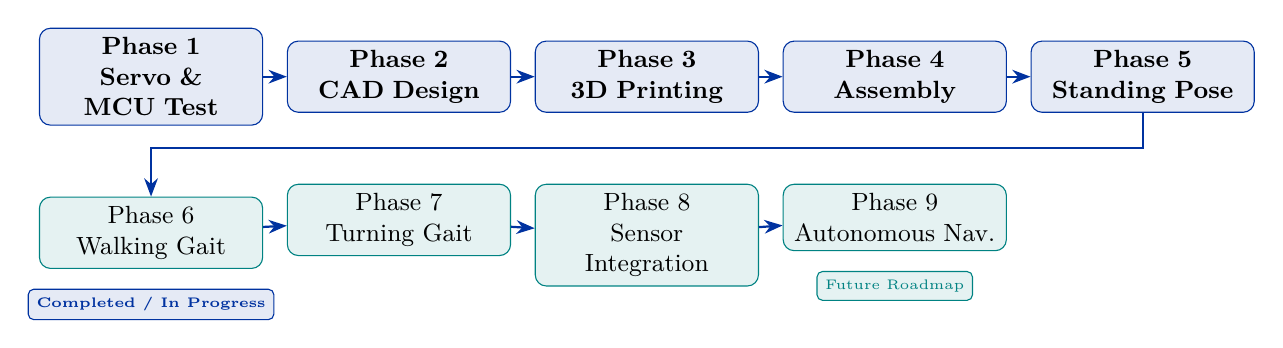
\begin{tikzpicture}[
  node distance=0.55cm and 0.3cm,
  block/.style={rectangle, draw=myblue, fill=myblue!10, rounded corners=4pt,
                text width=2.6cm, text centered, minimum height=0.75cm,
                font=\small\bfseries},
  future/.style={rectangle, draw=myteal, fill=myteal!10, rounded corners=4pt,
                 text width=2.6cm, text centered, minimum height=0.75cm,
                 font=\small},
  arrow/.style={thick, ->, >=Stealth, color=myblue}
]
  % Row 1: Phase 1 → 2 → 3 → 4 → 5  (left to right)
  \node[block]  (p1) {Phase 1\\Servo \& MCU Test};
  \node[block, right=of p1] (p2) {Phase 2\\CAD Design};
  \node[block, right=of p2] (p3) {Phase 3\\3D Printing};
  \node[block, right=of p3] (p4) {Phase 4\\Assembly};
  \node[block, right=of p4] (p5) {Phase 5\\Standing Pose};
  % Row 2: Phase 6 → 7 → 8 → 9  (left to right, aligned under row 1)
  \node[future, below=0.9cm of p1] (p6) {Phase 6\\Walking Gait};
  \node[future, below=0.9cm of p2] (p7) {Phase 7\\Turning Gait};
  \node[future, below=0.9cm of p3] (p8) {Phase 8\\Sensor Integration};
  \node[future, below=0.9cm of p4] (p9) {Phase 9\\Autonomous Nav.};
  % Row 1 arrows left→right
  \draw[arrow] (p1)--(p2); \draw[arrow] (p2)--(p3);
  \draw[arrow] (p3)--(p4); \draw[arrow] (p4)--(p5);
  % Phase 5 drops down then left to Phase 6
  \draw[arrow] (p5.south) -- ++(0,-0.45) -| (p6.north);
  % Row 2 arrows left→right
  \draw[arrow] (p6)--(p7); \draw[arrow] (p7)--(p8); \draw[arrow] (p8)--(p9);
  % Legend
  \node[draw=myblue, fill=myblue!10, rounded corners=2pt,
        font=\tiny\bfseries, inner sep=3pt, below=0.25cm of p6]
        {\color{myblue} Completed / In Progress};
  \node[draw=myteal, fill=myteal!10, rounded corners=2pt,
        font=\tiny, inner sep=3pt, below=0.25cm of p9]
        {\color{myteal} Future Roadmap};
\end{tikzpicture}
\end{tcolorbox}

\subsection{Phase 1 --- Component Verification}

Before mechanical construction, each component was tested in isolation. The ESP32
was verified with an LED blink sketch. The PCA9685 was tested using an I2C
scanner, confirming address \texttt{0x40}. All eight SG90 servos were tested
directly on ESP32 GPIO18. A critical issue was encountered: servos were not
moving when controlled through the PCA9685. Diagnosis revealed the
\textbf{V+ power rail measured only 0.10~V} --- the servo rail had no external
5~V supply. This was resolved by wiring 5~V directly to the V+ terminal.

\subsection{Phase 2 --- CAD Design}

With dimensions finalised (see Section~\ref{sec:mechanical}), the team modelled
each component in FreeCAD using the Part Design workbench. Bodies were created
for: Core Plate, Head Box, Upper Leg, Lower Leg, Servo Mount, and Assembly. The
Core Plate was modelled first as it defines all hip servo mount positions.

\subsection{Phase 3 --- 3D Printing}

All components were exported as STL files and sliced with standardised settings:
0.2~mm layer height, 40\% infill, 4 perimeter walls, 0.4~mm nozzle. Core Plate
and Head Box were printed in PLA+ for rigidity; leg segments in PETG for
flexibility and impact resistance.

\subsection{Phase 4 \& 5 --- Assembly and Standing Pose}

Servo horns were attached to each SG90 and press-fitted into printed mounts. All
eight servos were connected to the PCA9685 per the channel mapping (CH0--CH8).
The initial standing pose was achieved by calibrating each servo's neutral angle
to position the legs vertically, distributing the robot's weight evenly.

\clearpage
% ============================================================
%  5. ELECTRONICS ARCHITECTURE
% ============================================================
\section{Electronics Architecture}\label{sec:electronics}

\subsection{Component Overview}

The electronics stack has four layers: the \textbf{ESP32} as central controller,
the \textbf{PCA9685} as servo driver (I2C), \textbf{eight SG90 servos} as
actuators, and an \textbf{external 5~V supply} for the servo rail.

\begin{center}
\begin{tabular}{|l|l|l|}
\hline
\textbf{Component} & \textbf{Qty} & \textbf{Role} \\
\hline
ESP32 Dev Board & 1 & Main controller (I2C master) \\
PCA9685 16-ch PWM Driver & 1 & Servo PWM generation (I2C slave) \\
SG90 Servo Motor & 8 & Actuators (legs + head) \\
5V External Power Supply & 1 & Servo rail power \\
\hline
\end{tabular}
\end{center}

\subsection{ESP32 to PCA9685 I2C Connections}

\begin{center}
\begin{tabular}{|c|c|}
\hline
\textbf{ESP32 Pin} & \textbf{PCA9685 Pin} \\
\hline
3.3V   & VCC \\
GND    & GND \\
GPIO21 & SDA \\
GPIO22 & SCL \\
\hline
\end{tabular}
\end{center}

The PCA9685 uses 3.3~V logic but its servo rail (V+) must receive a
\textbf{separate external 5~V supply}. Power for VCC and V+ are electrically
isolated; the only shared connection is GND.

\subsection{Servo Channel Mapping}

\begin{center}
\renewcommand{\arraystretch}{1.4}
\begin{tabular}{|>{\bfseries}c|l|c|}
\hline
\rowcolor{myblue!15}\textbf{Channel} & \textbf{Servo Function} & \textbf{Type} \\
\hline
CH0 & Front Left Hip   & Hip  \\
\rowcolor{gray!8}
CH1 & Front Left Knee  & Knee \\
CH2 & Front Right Hip  & Hip  \\
\rowcolor{gray!8}
CH3 & Front Right Knee & Knee \\
CH4 & Rear Left Hip    & Hip  \\
\rowcolor{gray!8}
CH5 & Rear Left Knee   & Knee \\
CH6 & Rear Right Hip   & Hip  \\
\rowcolor{gray!8}
CH7 & Rear Right Knee  & Knee \\
CH8 & Head Rotation    & Head \\
\hline
\end{tabular}
\end{center}

\subsection{Servo Power Rail --- Critical Discovery}

During Phase~1 testing, an important real-world debugging experience was
encountered:

\begin{tcolorbox}[
  colback=myamber!10, colframe=myamber,
  arc=4pt, boxrule=0.5pt,
  colbacktitle=myamber, coltitle=white,
  title={\bfseries Critical Finding: PCA9685 V+ Power Rail Issue}
]
\textbf{Symptom:} All 8 servos unresponsive when controlled via PCA9685.\\[4pt]
\textbf{I2C Diagnosis:} Scanner confirmed PCA9685 at address \texttt{0x40} ---
ESP32, I2C bus, and chip all functioning correctly.\\[4pt]
\textbf{Root Cause:} V+ rail measured \textbf{0.10~V} (expected 4.8--5.2~V).
Servo power rail not connected to external 5~V supply.\\[4pt]
\textbf{Resolution:} Connect 5~V directly to PCA9685 V+ terminal. Servos
responded immediately.\\[4pt]
\textbf{Lesson:} Always verify servo rail voltage before suspecting firmware
or I2C issues.
\end{tcolorbox}

\subsection{Direct Servo Testing Connections}

\begin{center}
\begin{tabular}{|l|l|}
\hline
\textbf{Servo Wire}      & \textbf{ESP32 Connection} \\
\hline
Signal (Orange/Yellow)  & GPIO18   \\
VCC (Red)               & VIN (5V) \\
GND (Brown/Black)       & GND      \\
\hline
\end{tabular}
\end{center}








% ── Fig. 2 ────────────────────────────────────────────────
\begin{figure}[H]
  \centering
  \vspace{10cm}
  \caption{ESP32 and PCA9685 wiring setup}
  \label{fig:wiring}
\end{figure}




\clearpage
% ============================================================
%  6. MECHANICAL ARCHITECTURE & CAD DESIGN
% ============================================================
\section{Mechanical Architecture \& CAD Design}\label{sec:mechanical}

\subsection{Structural Overview}

The quadruped's structure consists of two assemblies: the \textbf{Head Box}
(housing all electronics) and the \textbf{Core Plate} (central chassis mounting
all four hip servos). Each leg has two links --- an \textbf{Upper Leg} driven by
the hip servo and a \textbf{Lower Leg} driven by the knee servo.

\subsection{Component Dimensions}

\begin{center}
\begin{tabularx}{\textwidth}{|l|l|X|}
\hline
\textbf{Component} & \textbf{Dimensions (mm)} & \textbf{Notes} \\
\hline
Core Plate  & 110 $\times$ 85 $\times$ 4  & 4 hip mounts + 1 head servo mount \\
Head Box    & 85 $\times$ 65 $\times$ 45  & Wall 2.5 mm; ESP32, PCA9685, switch \\
Upper Leg   & 45 $\times$ 10 $\times$ 5  & $\times$4 total \\
Lower Leg   & 55 $\times$ 10 $\times$ 5  & $\times$4 total \\
Servo Mount & Custom                       & Press-fit for SG90 body \\
\hline
\end{tabularx}
\end{center}

\subsection{Servo Placement --- Top View}

\begin{tcolorbox}[
  colback=gray!15, colframe=gray!40,
  arc=4pt, boxrule=0.5pt,
  title={\bfseries\color{myblue} Robot Top-View --- Servo Layout Diagram}
]
\centering
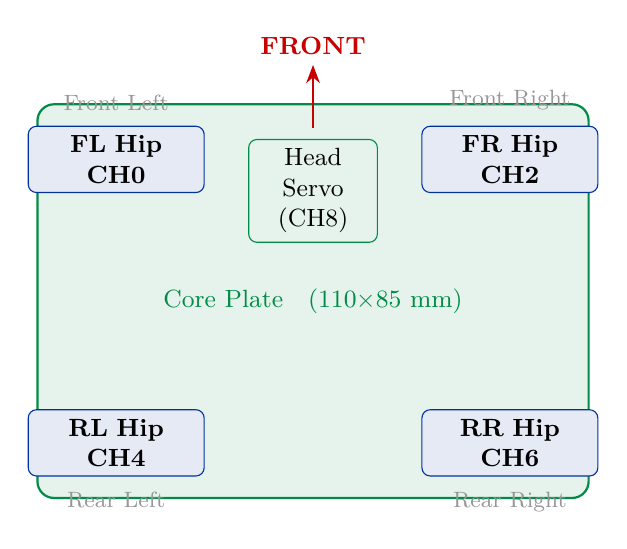
\begin{tikzpicture}[
  servo/.style={rectangle, draw=myblue, fill=myblue!10, text width=2.0cm,
                text centered, minimum height=0.7cm, rounded corners=3pt,
                font=\small\bfseries},
  plate/.style={rectangle, draw=mygreen, fill=mygreen!10, text width=1.4cm,
                text centered, minimum height=0.7cm, rounded corners=3pt,
                font=\small},
  lbl/.style={font=\footnotesize\color{footergray}}
]
  \draw[mygreen, thick, rounded corners=6pt, fill=mygreen!10]
    (-3.5,-2.5) rectangle (3.5,2.5);
  \node[font=\small\color{mygreen}] at (0,0) {Core Plate\quad(110$\times$85 mm)};
  \node[plate] at (0, 1.4) {Head Servo\\(CH8)};
  \node[servo] (fl) at (-2.5, 1.8) {FL Hip\\CH0};
  \node[servo] (fr) at ( 2.5, 1.8) {FR Hip\\CH2};
  \node[servo] (rl) at (-2.5,-1.8) {RL Hip\\CH4};
  \node[servo] (rr) at ( 2.5,-1.8) {RR Hip\\CH6};
  \node[lbl, above=2pt of fl] {Front Left};
  \node[lbl, above=2pt of fr] {Front Right};
  \node[lbl, below=2pt of rl] {Rear Left};
  \node[lbl, below=2pt of rr] {Rear Right};
  \draw[->, >=Stealth, myred, thick] (0,2.2)--(0,3.0)
    node[above, font=\small\bfseries\color{myred}] {FRONT};
\end{tikzpicture}
\end{tcolorbox}

\subsection{FreeCAD Design Workflow}

\begin{enumerate}[label=\arabic*., itemsep=4pt]
  \item \textbf{Core Plate} --- Base dimensions with servo mounting pockets.
  \item \textbf{Head Servo Mount} --- Centred on Core Plate; controls head rotation.
  \item \textbf{Hip Servo Mounts} --- Four symmetric pockets at FL, FR, RL, RR.
  \item \textbf{Upper Leg} --- 45~mm link with servo horn connection hole.
  \item \textbf{Lower Leg} --- 55~mm link with foot pad boss at terminal end.
  \item \textbf{Head Box} --- Enclosure around ESP32 and PCA9685 PCB footprints.
  \item \textbf{Assembly} --- All bodies assembled with correct spacing.
\end{enumerate}












% ── Fig. 6 ────────────────────────────────────────────────
\begin{figure}[H]
  \centering
  \vspace{10cm}
  \caption{Full Assembly in Ideamaker}
  \label{fig:cad_assembly}
\end{figure}

% ============================================================
%  7. PRODUCTS MADE (PRINTED PARTS)
% ============================================================
\section{Products Made (Printed Parts)}

\subsection{Printed Part Summary}

\begin{center}
\begin{tabularx}{\textwidth}{|l|l|X|c|}
\hline
\textbf{Part}   & \textbf{Material} & \textbf{Dimensions}               & \textbf{Qty} \\
\hline
Core Plate      & PLA+  & 110 $\times$ 85 $\times$ 4 mm             & 1 \\
Head Box        & PLA+  & 85 $\times$ 65 $\times$ 45 mm (wall 2.5)  & 1 \\
Upper Leg       & PETG  & 45 $\times$ 10 $\times$ 5 mm              & 4 \\
Lower Leg       & PETG  & 55 $\times$ 10 $\times$ 5 mm              & 4 \\
Servo Mount     & PLA+  & Custom (SG90 press-fit)                  & 9 \\
\hline
\end{tabularx}
\end{center}

\subsection{Core Plate}

The Core Plate is the central structural member --- a flat 110$\times$85~mm plate
with four symmetric hip servo pockets and one central head servo mount. The
4~mm thickness provides bending rigidity for the servo loads.

\subsection{Head Box}

The Head Box (85$\times$65$\times$45~mm, wall 2.5~mm) houses the ESP32, PCA9685,
and power switch, with provision for future sensor mounts.

\subsection{Leg Components}

Upper Leg (45~mm) and Lower Leg (55~mm) are PETG links, 10~mm wide and 5~mm
thick, with servo horn attachment holes at the joint ends.

% ── Fig. 10 ───────────────────────────────────────────────
\begin{figure}[H]
  \centering
  \vspace{10cm}
  \caption{3D Printed Leg Components (Material: PLA+)}
  \label{fig:legs}
\end{figure}

% ============================================================
%  8. ARDUINO PROGRAMMING
% ============================================================
\section{Arduino Programming}

\subsection{Development Environment}

All firmware was written using \textbf{Arduino IDE} with the ESP32 board support
package. Libraries used:
\begin{itemize}[itemsep=3pt]
  \item \texttt{ESP32Servo} --- direct servo control via GPIO PWM.
  \item \texttt{Wire} --- I2C communication for the PCA9685.
  \item \texttt{Adafruit\_PWMServoDriver} --- high-level PCA9685 control.
\end{itemize}

\subsection{Servo Test Code}

Each SG90 servo was tested individually on GPIO18 before PCA9685 integration:

\begin{lstlisting}[language=C++, caption={Servo Test Code (ESP32 direct GPIO18)}, label={lst:servotest}]
#include <ESP32Servo.h>

Servo myServo;

void setup() {
  myServo.attach(18);   // Signal on GPIO18
}

void loop() {
  myServo.write(0);     // 0 degrees
  delay(1000);
  myServo.write(90);    // 90 degrees (neutral)
  delay(1000);
  myServo.write(180);   // 180 degrees
  delay(1000);
}
\end{lstlisting}

\subsection{PCA9685 I2C Scanner}

Before running servo control through the PCA9685, the I2C bus was scanned to
confirm the PCA9685 address:

\begin{lstlisting}[language=C++, caption={I2C Scanner --- PCA9685 Address Verification}, label={lst:i2cscan}]
#include <Wire.h>

void setup() {
  Wire.begin(21, 22);   // SDA=GPIO21, SCL=GPIO22
  Serial.begin(115200);
  Serial.println("Scanning I2C bus...");
  for (byte addr = 1; addr < 127; addr++) {
    Wire.beginTransmission(addr);
    if (Wire.endTransmission() == 0) {
      Serial.print("I2C device found at 0x");
      if (addr < 16) Serial.print("0");
      Serial.println(addr, HEX);
    }
  }
  Serial.println("Scan complete.");
}

void loop() {}
\end{lstlisting}

Expected serial monitor output:

\begin{lstlisting}[language={}, caption={I2C Scan Output --- Serial Monitor}, label={lst:i2coutput}]
Scanning I2C bus...
I2C device found at 0x40
Scan complete.
\end{lstlisting}

Address \texttt{0x40} is the factory-default PCA9685 I2C address (all A0--A5
pins low), confirming SDA/SCL wiring and chip operation.

\subsection{PCA9685 Servo Control}

Once the V+ issue was resolved (Section~\ref{sec:electronics}), all eight servos
were driven through the PCA9685:

\begin{lstlisting}[language=C++, caption={PCA9685 All-Channel Servo Sweep}, label={lst:pca9685sweep}]
#include <Wire.h>
#include <Adafruit_PWMServoDriver.h>

Adafruit_PWMServoDriver pwm = Adafruit_PWMServoDriver(0x40);

#define SERVOMIN  150   // ~0 degrees @ 50Hz
#define SERVOMAX  600   // ~180 degrees @ 50Hz
#define SERVO_FREQ 50

uint16_t angleToPulse(int angle) {
  return map(angle, 0, 180, SERVOMIN, SERVOMAX);
}

void setup() {
  Wire.begin(21, 22);
  pwm.begin();
  pwm.setOscillatorFrequency(27000000);
  pwm.setPWMFreq(SERVO_FREQ);
  delay(10);
}

void loop() {
  for (int ch = 0; ch < 9; ch++)
    pwm.setPWM(ch, 0, angleToPulse(90));   // all neutral
  delay(2000);
  for (int ch = 0; ch < 9; ch++)
    pwm.setPWM(ch, 0, angleToPulse(45));   // all 45 deg
  delay(2000);
}
\end{lstlisting}

% ============================================================
%  9. RESULTS & TESTING
% ============================================================
\section{Results \& Testing}

\subsection{I2C Communication Verification}

The PCA9685 I2C address was confirmed as \texttt{0x40} using the scanner
(Listing~\ref{lst:i2cscan}), validating the full chain:
ESP32 $\rightarrow$ GPIO21/22 $\rightarrow$ SDA/SCL $\rightarrow$ PCA9685.

\subsection{Power Rail Diagnosis and Resolution}

As documented in Section~\ref{sec:electronics}, the V+ rail measured 0.10~V
initially. After connecting an external 5~V supply, it measured 4.92--5.05~V.
All servos responded immediately.

\subsection{Individual Servo Testing Results}

All eight SG90 servos were tested using the direct sweep code
(Listing~\ref{lst:servotest}):

\begin{center}
\begin{tabularx}{\textwidth}{|c|X|c|c|}
\hline
\textbf{Servo} & \textbf{Function} & \textbf{0$^\circ$} & \textbf{180$^\circ$} \\
\hline
1 & Front Left Hip (CH0)   & \color{mygreen}Pass & \color{mygreen}Pass \\
2 & Front Left Knee (CH1)  & \color{mygreen}Pass & \color{mygreen}Pass \\
3 & Front Right Hip (CH2)  & \color{mygreen}Pass & \color{mygreen}Pass \\
4 & Front Right Knee (CH3) & \color{mygreen}Pass & \color{mygreen}Pass \\
5 & Rear Left Hip (CH4)    & \color{mygreen}Pass & \color{mygreen}Pass \\
6 & Rear Left Knee (CH5)   & \color{mygreen}Pass & \color{mygreen}Pass \\
7 & Rear Right Hip (CH6)   & \color{mygreen}Pass & \color{mygreen}Pass \\
8 & Rear Right Knee (CH7)  & \color{mygreen}Pass & \color{mygreen}Pass \\
9 & Head Rotation (CH8)    & \color{mygreen}Pass & \color{mygreen}Pass \\
\hline
\end{tabularx}
\end{center}

All 8 servos completed the full range 0°--90°--180° without issues.

\subsection{Development Phase Status}

\begin{center}
\begin{tabular}{|c|l|l|}
\hline
\textbf{Phase} & \textbf{Description} & \textbf{Status} \\
\hline
1 & Component verification        & \color{mygreen}\bfseries Complete \\
2 & CAD design in FreeCAD         & \color{mygreen}\bfseries Complete \\
3 & 3D printing all parts         & \color{mygreen}\bfseries Complete \\
4 & Servo calibration             & \color{mygreen}\bfseries Complete \\
5 & Standing pose                 & \color{mygreen}\bfseries Complete \\
6 & Walking gait                  & \color{myamber}\bfseries In Progress \\
7 & Turning gait                  & \color{myamber}\bfseries Planned \\
8 & Sensor integration            & \color{myamber}\bfseries Planned \\
9 & Autonomous navigation         & \color{myamber}\bfseries Future \\
\hline
\end{tabular}
\end{center}


% ── Fig. 12 ───────────────────────────────────────────────
\begin{figure}[H]
  \centering
  \vspace{10cm}
  \caption{Partially Assembled Quadruped Robot}
  \label{fig:assembly}
\end{figure}

\clearpage
% ============================================================
%  10. CONCLUSION
% ============================================================
\section{Conclusion}

This project has been a comprehensive experience in legged robot development ---
from component verification through mechanical design, additive manufacturing,
and embedded programming. Group-E has successfully built the hardware and
software stack for an 8-DOF quadruped robot across three engineering disciplines.

From an \textbf{electronics perspective}, the project reinforced systematic
debugging skills. The PCA9685 V+ rail issue --- diagnosed through I2C scanning
and multimeter probing --- exemplifies real-world troubleshooting. All eight
servos and the confirmed I2C address \texttt{0x40} provide a solid foundation.

From a \textbf{mechanical design perspective}, parametric CAD in FreeCAD taught
servo mount constraints, press-fit tolerancing, and STL export for manufacturing.

From a \textbf{3D printing perspective}, material selection (PLA+ vs PETG),
slicer optimisation, and print quality assessment gave hands-on applied knowledge
building on the theory covered in this report.

Looking ahead: walking gait (Phase~6), turning (Phase~7), sensor integration
(Phase~8), and autonomous navigation (Phase~9). The ESP32's Wi-Fi also enables
remote teleoperation. Group-E is proud to have contributed a fully functional
quadruped robot platform to the WTL \& MeitY programme at CGEC.

% ============================================================
%  BIBLIOGRAPHY
% ============================================================
\begin{thebibliography}{9}

\bibitem{prevbatch}
  \textit{Previous Batch Project Report --- 3D Printing and Embedded Systems},
  CGEC, Department of ECE, WTL \& MeitY Project,
  Cooch Behar, West Bengal, 2024.

\bibitem{esp32docs}
  Espressif Systems,
  \textit{ESP32 Technical Reference Manual}, v5.3,
  Espressif Systems, 2024.

\bibitem{pca9685}
  NXP Semiconductors,
  \textit{PCA9685 16-channel, 12-bit PWM I2C-bus LED controller},
  Product data sheet Rev.\ 4, NXP, 2015.

\bibitem{mg90s}
  Tower Pro,
  \textit{SG90 Metal Gear Micro Servo Datasheet},
  Tower Pro Co.\ Ltd., 2020.

\bibitem{freecad}
  FreeCAD Community,
  \textit{FreeCAD: Your Own 3D Parametric Modeler},
  \url{https://www.freecad.org}, 2024.

\end{thebibliography}

\end{document}
